\documentclass{juliacon}
\setcounter{page}{1}

\begin{document}

\newcommand{\R}{\ensuremath{\mathbb{R}}}
\newcommand{\RE}{RangeEnclosures}
\newcommand{\pkgl}[2]{\href{#1}{\pkg{#2}}}
\newcommand{\pkg}[1]{\texttt{#1.jl}}

% **************GENERATED FILE, DO NOT EDIT**************

\title{RangeEnclosures.jl: A framework to bound function ranges}

\author[1]{Luca Ferranti}
\author[2]{Marcelo Forets}
\author[3]{Christian Schilling}
\affil[1]{University of Vaasa, Finland}
\affil[2]{Universidad de la Rep\'{u}blica, Uruguay}
\affil[3]{Aalborg University, Denmark}

\keywords{range enclosure, rigorous computing, reachability analysis, interval methods}

\hypersetup{
pdftitle = {RangeEnclosures.jl: A framework to bound function ranges},
pdfsubject = {JuliaCon 2022 Proceedings},
pdfauthor = {Luca Ferranti, Marcelo Forets, Christian Schilling},
pdfkeywords = {range enclosure, rigorous computing, reachability analysis, interval methods},
}



\maketitle

\begin{abstract}
Computing the range of a function is needed in several application domains. During the past decades, several algorithms to compute or approximate the range have been developed, each with its own merits and limitations.
Motivated by this, we introduce \pkg{\RE}, a unified framework to bound the range of univariate and multivariate functions. In addition to its own algorithms, the package allows to easily integrate third-party algorithms, offering a unified interface that can be used across different domains and allows to easily benchmark different approaches.
\end{abstract}



\section{Introduction}

Given a function $f: \mathcal{D} \to \R$ over a domain $\mathcal{D}\subseteq\R$, the \emph{range} (or image) is the set $\mathcal{R}=\{y\in\R \mid \exists x\in\mathcal{D}: f(x)=y\}$. In practical applications, we are interested in determining the \textit{interval range} of $f$, i.e., the smallest interval containing $\mathcal{R}$. Unfortunately, computing the interval range of a multivariate function is NP-hard~\cite{kreinovich2002range}.

For this reason, we practically seek an \textit{enclosure} $\mathcal{E}\supseteq\mathcal{R}$ of the interval range. A standard method to obtain an enclosure is to evaluate the function with interval arithmetic~\cite{moore2009introduction}, which however often produces a wide overestimation due to issues such as the dependency problem and the wrapping effect. For this 
reason, different algorithms have been developed over the past decades~\cite{de2004affine,hansen2003global}, but each comes with its own strengths and weaknesses. This is visualized in Fig.~\ref{fig:enclosure_2D}, where the enclosure obtained with plain interval arithmetic (natural enclosure) is compared to the result of a branch-and-bound algorithm. In general, when choosing an algorithm to compute a function enclosure, a trade-off between accuracy and computational efficiency has to be made.

\smallskip

We present \pkgl{https://github.com/JuliaReach/RangeEnclosures.jl}{\RE}, a Julia~\cite{BezansonEKS17} package offering a unified framework to bound the range of univariate and multivariate functions. The package comes with built-in solvers but also seamlessly integrates solvers defined in third-party libraries. This allows to easily compare different approaches.



\section{A tour through \RE}

In this section we give a quick overview of the API to bound function ranges. The package offers several solvers for this purpose, such as natural (interval) enclosure, mean-value form~\cite{moore2009introduction}, Moore-Skelboe algorithm~\cite{hansen2003global}, and Taylor models~\cite{benet2019taylormodels}, or polynomial optimization~\cite{legat2017sos}. The full list of implemented solvers can be found in the package documentation\footnote{\url{https://juliareach.github.io/RangeEnclosures.jl/}}.


\subsection{The enclose API}

The \emph{\RE} API works through the function \texttt{enclose}.
The basic usage is via \texttt{enclose(f, D, solver; kwargs...)}, where \texttt{f} is the function whose range we want to bound, \texttt{D} is the domain over which we want to compute the range, \texttt{solver} is the solver used to compute the range (if no solver is specified, the package will default to the \texttt{NaturalEnclosure} solver), and \texttt{kwargs} are possible keyword arguments used by the solver.

\begin{figure}[tb]
    \centering
    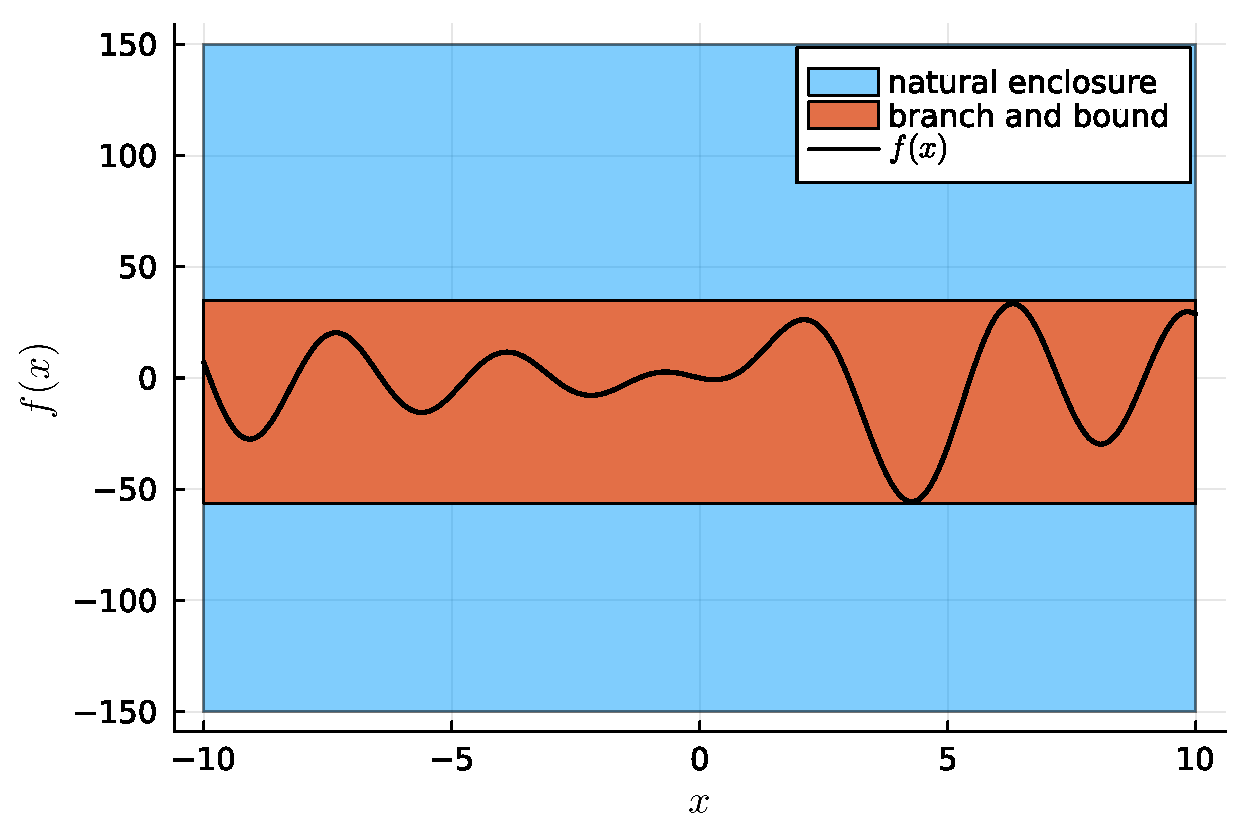
\includegraphics[width=\linewidth,height=6cm,keepaspectratio]{pic/enclosure_2D}
    \caption{Two enclosures of $f(x) = -\sum_{k=1}^5kx\sin(\frac{k(x-3)}{3})$.}
    \label{fig:enclosure_2D}
\end{figure}

In \emph{\RE}, the \texttt{solver} is an instance of a struct that must be a subtype of \texttt{AbstractEnclosureAlgorithm}.
If a user wants to add a new solver, they just have to add a new struct, say, \texttt{MyEnclosure} and extend the method \texttt{enclose}.
%
\begin{lstlisting}[language=Julia]
enclose(f::Function, D::Union{Interval, IntervalBox},
        solver::MyEnclosure; kwargs...)
\end{lstlisting}

Note that \texttt{D} can be of type \texttt{Interval} for univariate ($n = 1$) functions or of type \texttt{IntervalBox} for multivariate ($n > 1$) functions.


\subsection{How to use the package}

Below we show Julia code to specify the motivating example from above as well as to compute a range enclosure. Here we use the solvers \texttt{NaturalEnclosure} and \texttt{BranchAndBoundEnclosure}.

\begin{lstlisting}[language=Julia]
julia> f(x) = -sum(k*x*sin(k*(x-3)/3) for k in 1:5);
julia> D = -10..10;
julia> enclose(f, D, NaturalEnclosure())
[-150, 150]
julia> enclose(f, D, BranchAndBoundEnclosure())
[-56.4232, 34.9988]
\end{lstlisting}


\paragraph*{Combining different solvers}

Sometimes there is no ``best'' solver, as one solver might give a tighter estimate of the range's upper bound and another solver might give a tighter estimate of the lower bound. In this case, the results can be combined. Consider the function $g(x) = x^2 - 2x + 1$ over the domain $D_g = [0, 4]$. We use the solvers \texttt{NaturalEnclosure} and the \texttt{MeanValueEnclosure}:

\begin{lstlisting}[language=Julia]
julia> g(x) = x^2 - 2*x + 1;
julia> Dg = 0..4;
julia> enclose(g, Dg, NaturalEnclosure())
[-7, 17]
julia> enclose(g, Dg, MeanValueEnclosure())
[-11, 13]
\end{lstlisting}

A better enclosure could be obtained by taking the intersection of the two results. This can be easily done in one command by passing a vector of solvers to \texttt{enclose}:

\begin{lstlisting}[language=Julia]
julia> enclose(g, Dg, [NaturalEnclosure(),
                       MeanValueEnclosure()])
[-7, 13]
\end{lstlisting}


\paragraph*{Using solvers based on external libraries}

Some of the available solvers are implemented in external libraries. To keep the start-up time of \emph{\RE}\ low, these libraries are not imported by default. To use the corresponding solver, the library needs to be manually loaded. For instance, the Moore-Skelboe algorithm is available upon loading the package \pkgl{https://github.com/JuliaIntervals/IntervalOptimisation.jl}{Intervaloptimisation}.

\begin{lstlisting}[language=Julia]
julia> import IntervalOptimisation
julia> enclose(g, Dg, MooreSkelboeEnclosure())
[-0.00191952, 9.00109]
\end{lstlisting}


\paragraph*{Multivariate functions}

The techniques generalize to multivariate functions. Note that the domain becomes an \texttt{IntervalBox} (instead of an \texttt{Interval}). For example, consider the bivariate function $h(x_1, x_2) = \sin(x_1) - \cos(x_2) - \sin(x_1)\cos(x_1)$ over the domain $D_h = [-5, 5] \times [-5, 5]$. Fig.~\ref{fig:enclosure_3D} visualizes the result.

\begin{lstlisting}[language=Julia]
julia> h(x) = sin(x[1]) - cos(x[2]) - sin(x[1]) * cos(x[1]);
julia> Dh = IntervalBox(-5..5, -5..5);
julia> enclose(h, Dh, BranchAndBoundEnclosure())
[-2.71068, 2.71313]
\end{lstlisting}

\begin{figure}[t]
    \centering
    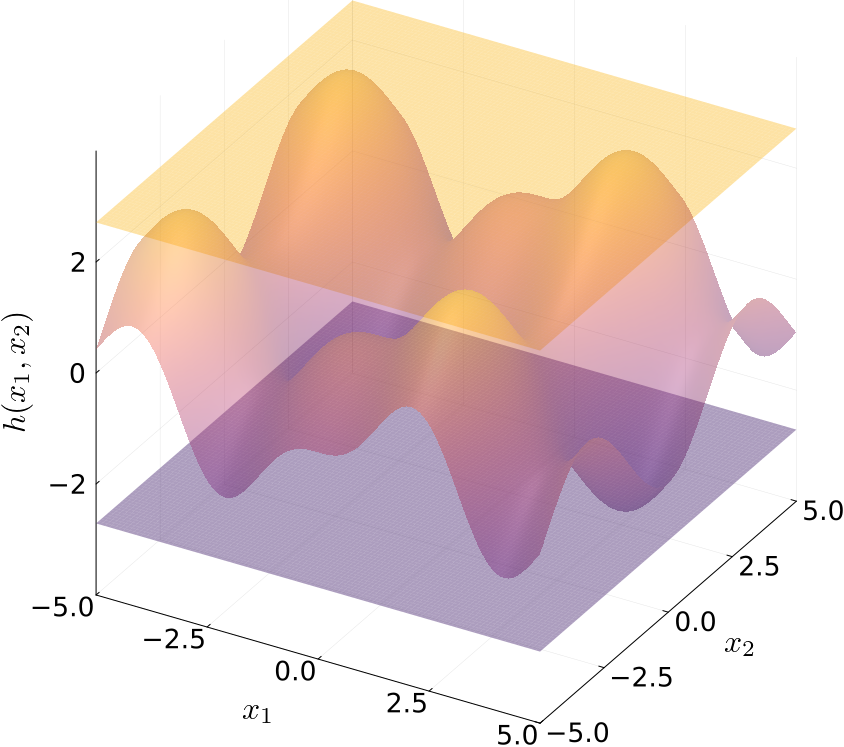
\includegraphics[width=\linewidth,height=48mm,keepaspectratio]{pic/enclosure_3D}
    \caption{An enclosure of the bivariate function $h$.}
    \label{fig:enclosure_3D}
\end{figure}



\section{Future Applications}
We envision applying the package to the domain of reachability analysis~\cite{althoff2021set, althoff2018implementation}. \emph{\RE}\ currently only supports functions with univariate range. To represent multivariate ranges as convex and non-convex sets, we plan to use \pkgl{https://github.com/JuliaReach/LazySets.jl}{LazySets}~\cite{ForetsS21}.

\section*{Acknowledgments}

This research was partly supported by DIREC - Digital Research Centre Denmark and the Villum Investigator Grant S4OS.


% **************GENERATED FILE, DO NOT EDIT**************

\bibliographystyle{juliacon}
\bibliography{ref.bib}


\end{document}
